% \begin{figure}[htbp] % positioning htbp: h = here; t = top; b bottom; p own page
% 	\centering
% 	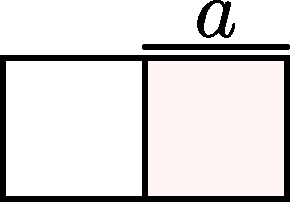
\includegraphics[scale=0.5]{KVdiagramm_a.pdf}
% 	\caption{KV-Diagramm für eine Variable}
% 	\label{KVdiag_a}
% \end{figure}
% 
% \begin{figure}[htbp] % positioning htbp: h = here; t = top; b bottom; p own page
% 	\centering
% 	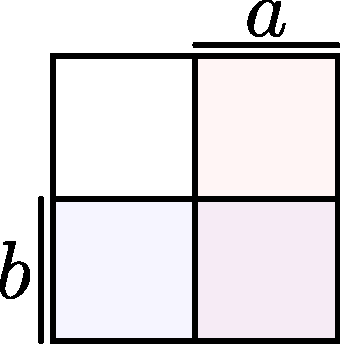
\includegraphics[scale=0.5]{KVdiagramm_ab.pdf}
% 	\caption{KV-Diagramm für zwei Variablen}
% 	\label{KVdiag_ab}
% \end{figure}
% 
% \begin{figure}[htbp] % positioning htbp: h = here; t = top; b bottom; p own page
% 	\centering
% 	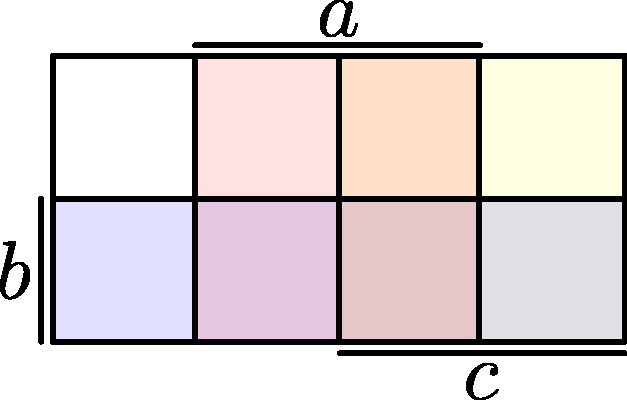
\includegraphics[scale=0.5]{KVdiagramm_abc.pdf}
% 	\caption{KV-Diagramm für drei Variablen}
% 	\label{KVdiag_abc}
% \end{figure}
% 
% \begin{figure}[htbp] % positioning htbp: h = here; t = top; b bottom; p own page
% 	\centering
% 	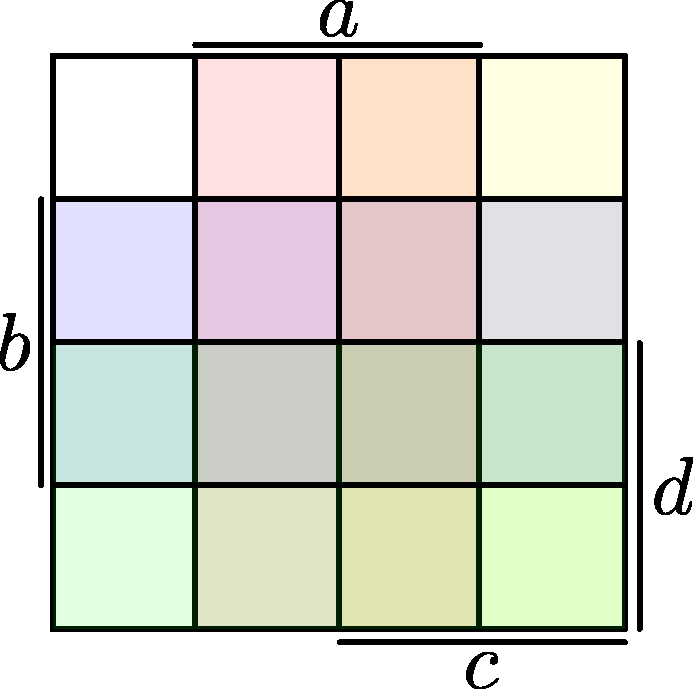
\includegraphics[scale=0.5]{KVdiagramm_abcd.pdf}
% 	\caption{KV-Diagramm für vier Variablen}
% 	\label{KVdiag_abcd}
% \end{figure}
